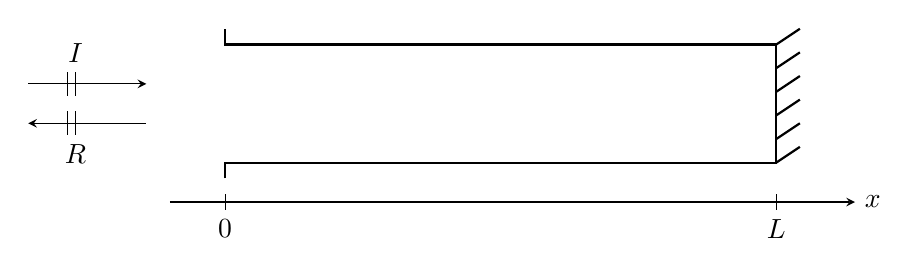
\begin{tikzpicture}[>=stealth]

	% waveguide
	\draw[thick] (0,.3) -- (0,.5) -- (7,.5) -- (7,2) -- (0,2) -- (0,2.2);
	\foreach \i in {0,...,5}{
		\draw[thick] (7,\i*0.3+0.5) -- ++(.3,.2);
	}
	
	% x axis
	\draw[->] (-.7,0) -- (8,0) node[right] {$x$};
	\draw (0,.1) -- ++(0,-.2) node[below] {$0$};
	\draw (7,.1) -- ++(0,-.2) node[below] {$L$};

	% waves
	% R
	\draw[<-] (-2.5,1) -- ++(1.5,0);
	\draw (-2,1.15) -- ++(0,-.3);
	\draw (-1.9,1.15) -- ++(0,-.3) node[below] {$R$};

	% I
	\draw[->] (-2.5,1.5) -- ++(1.5,0);
	\draw (-2,1.65) -- ++(0,-.3);
	\draw (-1.9,1.65) node[above] {$I$} -- ++(0,-.3);

\end{tikzpicture}

